\subsection{Communication between Micro-frontends}\label{subsection:background:micro-frontend:communication-patterns}

Micro-frontends should not depend on each other. Nevertheless, it is necessary to have communication between them. For example, if a user adds an item to a shopping cart in an e-commerce application, the product micro-frontend has to inform the shopping cart micro-frontend which item was added. To reduce the coupling between applications and development teams, keeping the communication between micro-frontends at a minimum is recommended. Before choosing a communication pattern, it is vital to know the type of communication. If communication between two micro-frontends or between the app shell and a micro-frontend is required, the communication can occur via the user interface. Other communication mechanisms, like the Broadcast Channel API provided by the browser, are helpful for state sharing or for passing on information to multiple micro-frontends.  \cite{book:2020:geers:background:micro-frontends:micro-frontends-in-action}

\bigskip

\noindent The communication can only happen via URL parameters when the micro-frontends are integrated using hyperlinks. Single-Page-Applications usually communicate via custom events and attribute changes of the components. \cite[100]{book:2020:geers:background:micro-frontends:micro-frontends-in-action} \cite[315-316]{book:2019:farrell:background:micro-frontends:web-components-in-action} A distinction can be made between \textbf{parent-to-fragment}, \textbf{fragment-to-parent} or \textbf{fragment-to-fragment} communication, where the term fragment is equivalent to a micro-frontend and the term parent is equivalent to the app shell. \cite{book:2020:geers:background:micro-frontends:micro-frontends-in-action} Figure \ref{fig:background:micro-frontend:communication:communication-patterns} shows the three types of communication in a diagram:

\ifshowImages
\begin{figure}[H]
    \centering
    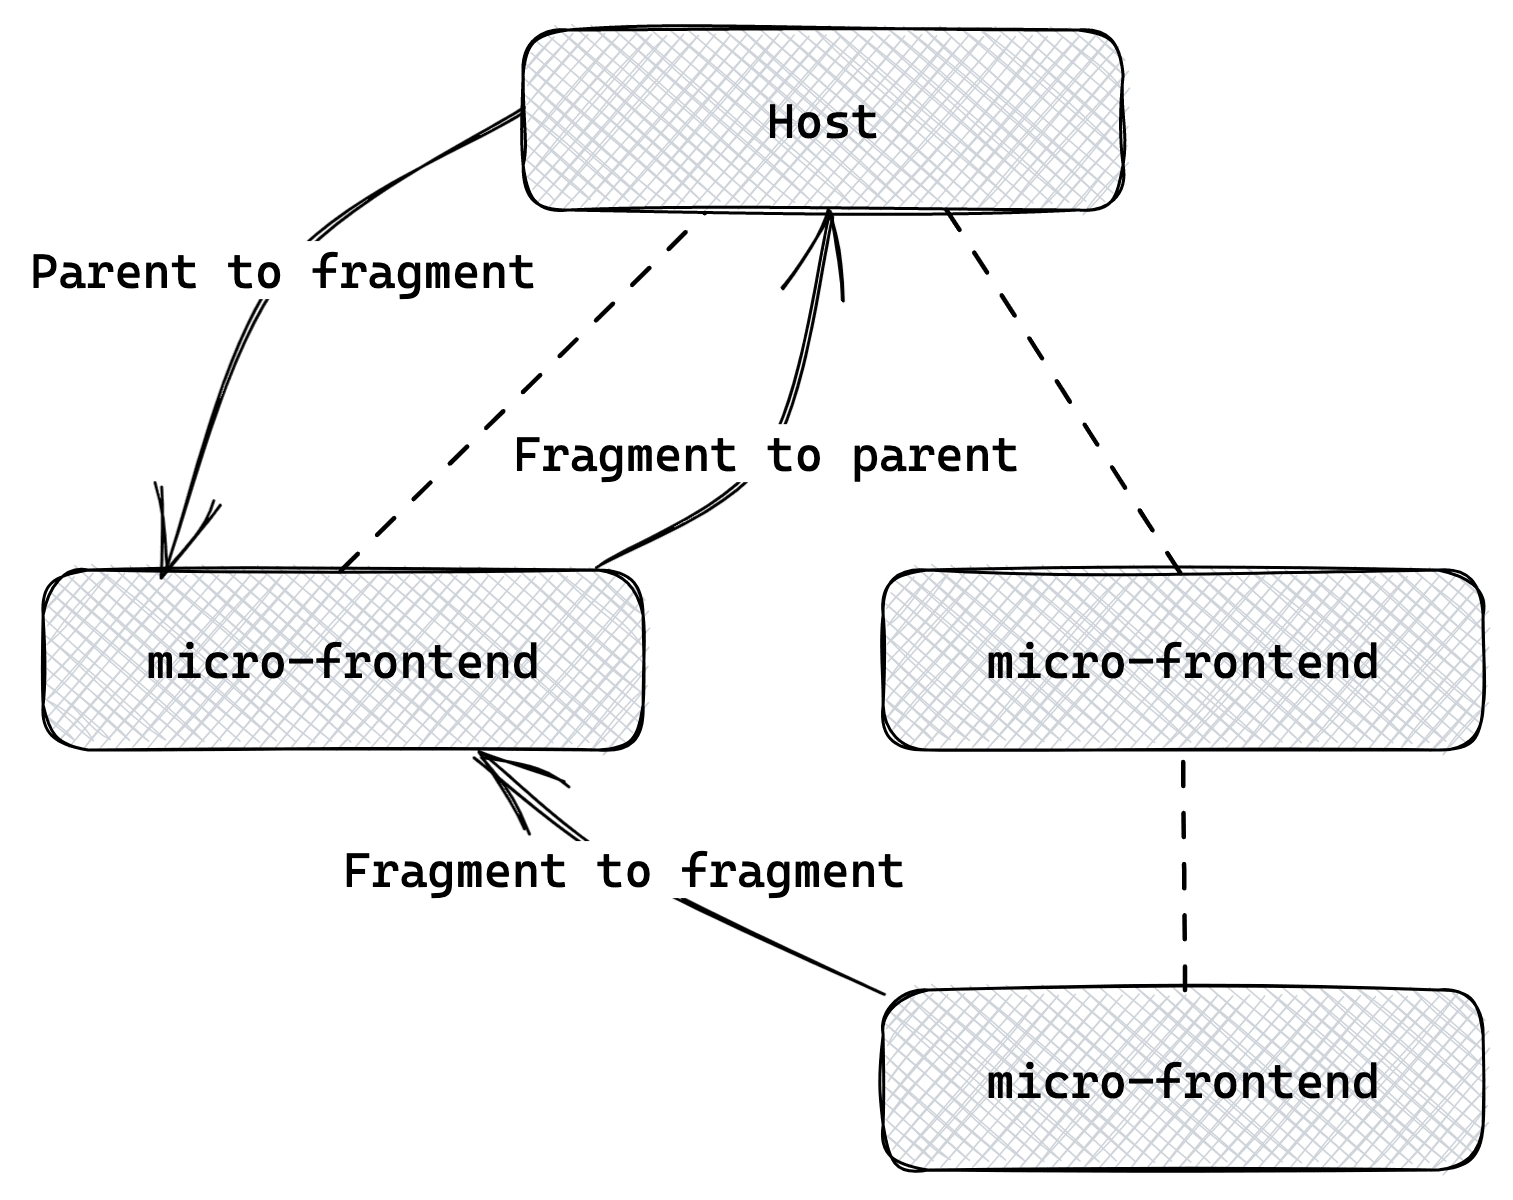
\includegraphics[width=0.5\linewidth]{images/background/communication/communication-patterns.png}
    \caption{Different forms of communication in micro-frontend architectures (Adapted from \cite[100]{book:2020:geers:background:micro-frontends:micro-frontends-in-action})}\label{fig:background:micro-frontend:communication:communication-patterns}
\end{figure}
\fi

\bigskip

\noindent Parent-to-fragment communication can happen via attribute changes when using Web Components. \cite[58-59]{book:2019:farrell:background:micro-frontends:web-components-in-action} To pass data from a micro-frontend to the app shell, custom events can be used. \cite[315]{book:2019:farrell:background:micro-frontends:web-components-in-action}, where the micro-frontend emits an event, that the app shell is subscribed to. \cite{book:2020:geers:background:micro-frontends:micro-frontends-in-action}

\bigskip

\noindent Fragment-to-fragment communication is required when two micro-frontends should communicate with each other. The changes in one micro-frontend should affect the other micro-frontend. This form of communication can be implemented in three ways: \cite[107-108]{book:2020:geers:background:micro-frontends:micro-frontends-in-action}

\begin{itemize}
    \item \textbf{Direct communication}: Direct communication is the most direct form of communication. One micro-frontend changes the attributes of its HTML elements with JavaScript. This approach is not recommended because it introduces high coupling between two micro-frontends. One micro-frontends needs to know the implementation details of the other micro-frontend. This implementation makes it difficult to change the implementation of one micro-frontend without breaking the other micro-frontend. Moreover, this breaks one characteristic of micro-frontends, which are independent and autonomous development and deployment.
    \item \textbf{Orchestration via a parent}: The app shell is responsible for communicating between micro-frontends when using this approach. One micro-frontend emits an event, which is intercepted by the application shell, and the application shell sends the event to the target micro-frontend. This approach allows the micro-frontends to be completely decoupled, but every micro-frontend must adapt to communication changes.
    \item \textbf{Event-Bus/broadcasting}: Instead of direct communication between micro-frontends or indirect communication via the application shell, a micro-frontend can publish an event on a central event bus. The other micro-frontends can subscribe to the events and react accordingly. This pattern is described as publish/subscribe mechanism, drastically reducing the coupling between micro-frontends. No micro-frontend needs information about the other micro-frontends, allowing perfect parallel development.
\end{itemize}
